\chapter{相互独立的序列型数据的隐私属性推测模型及其应用}
\label{chap:inference-attack-on-norelated-sequenced-data}

\section{引言}\label{sec:intro}

随着测序技术的进步,人们现在能够更轻松,更便宜地对其DNA进行测序。人类基因组数据已变得越来越可负担和可用。例如,在1000 Genomes项目\cite{gpc2015global}中,数千名匿名参与者将他们的DNA捐献给了生物医学和精准医学研究。美国、英国、加拿大、法国和中国政府也出于医学和其他原因启动了基因组数据收集项目。此外,越来越多的人通过23andMe.com、PatientsLikeMe.com和Ancestry.com等网站在线分享他们的基因组数据,或是为了娱乐,或是为了寻找亲人。另一方面,可以通过他或她的DNA来识别一个人。基因组数据还可用于识别特定的性状和疾病。然而,基因组数据可用性的提高带来了更加突出的安全和隐私挑战。一旦这些数据被披露或滥用,一个人就可能会面临就业、保险、教育等多方面的歧视风险\cite{eeoc2008genetic}。

实际上,许多研究结果和实际案例已经引起人们对基因组数据的机密性和隐私性的担忧。在某些情况下,以任何方式收集的基因组数据仍可能以各种方式暴露个人的敏感信息。例如,Sweeney等\cite{sweeney2013identifying}通过将个人基因组计划中不公开的姓名和联系信息链接起来,重新识别个体;Gymrek等\cite{gymrek2013identifying}通过分析Y染色体上的短串联重复序列,重新识别个体。全基因组关联研究(GWAS)的结果可用于识别个体\cite{cai2015deterministic}。某些疾病的易感性\cite{shringarpure2015privacy}和外观特征\cite{walsh2011irisplex}也可以从基因组数据中推断出来。个人基因组数据的泄露不仅会对其个人隐私造成威胁,而且还会以家族身份\cite{rohlfs2012familial}或有关亲属基因型信息的形式对其亲属的隐私造成威胁\cite{humbert2013addressing}。最近,已经证实遗传学家可以从他或她的基因组数据中恢复特定个体的面孔\cite{hess2017controversial}。共享的基因组数据也有可能被恶意机构滥用\cite{scutti2018what}。

情况可能更糟。为了保护个人自身的基因组隐私,通常他或她可以选择删除或隐藏其基因型的某些部分\cite{shi2017overview},只向第三方(如医院或基因组研究机构)共享部分基因组数据。许多没有亲戚关系的人可以通过这种方式共享他们的基因组数据似乎是安全的。但是,这并不有效。在这项工作中,我们将展示对手可以从该个体的共享部分基因组数据和其他公开可用的基因组数据中稳健地重建个体的基因组数据。

在本文中,我们将揭示两种用于重构单个基因型序列的推理攻击策略:一种基于改进的离散隐马尔可夫模型(iHMM),另一种基于回归卷积神经网络(RCNN)模型。这些推理攻击模型既考虑了观察到的受害者基因组数据,也考虑了公开可用的基因组数据。我们还将提出度量标准,以量化受害者的基因组隐私以及有关不正确性、不确定性和隐私损失的攻击的严重程度。与Samani等先前的工作\cite{samani2015quantifying}相比,我们的贡献如下:
\begin{itemize}
	\item 我们将提出一个针对基因组隐私推理攻击的统一对抗模型,目的是从受害者部分观察到的基因组数据中重建不相关个体的基因型序列。
	\item 我们将提出一种针对不相关个体的基因组隐私推理攻击策略,该策略利用IMPUTE2\cite{howie2009flexible}中单核苷酸多态性(SNPs)和抽样重组模型方法进行关联。
	\item	我们将展示一种采用RCNN的针对不相关个体的基因组隐私推理攻击策略,并研究在基因组隐私攻击背景下机器学习(例如RCNN)的大规模功能。
	\item 我们将从互信息的角度来评估推理攻击能力,量化基因组隐私,这代表攻击者信息不确定性的降低和受害者对攻击者隐私损失的增加。
	\item 与以往的工作相比,我们的结果具有更高的准确性,对推断的基因组数据的不确定性更低,对攻击者的隐私信息损失更大。
\end{itemize}

本文的其余部分组织如下。首先,第\ref{sec:relat}节将包括对先前相关作品的简要概述。接下来,第\ref{sec:back}节将介绍我们工作的一些基本背景。第\ref{sec:adver}节将讨论对手模型和评估指标。推理攻击策略的框架和细节将在第\ref{sec:infer}节中给出。在第\ref{sec:resul}节中,将对提出的推理攻击策略进行评估,并引入度量标准来量化基因组数据的隐私。最后,利用第\ref{sec:concl}节对本文进行了总结。

\section{相关工作}\label{sec:relat}
\subsection{基因序列隐私推测攻击}

推理攻击利用可用数据通过数据分析来推断潜在的私人信息\cite{en2018inference},是一种非常有效的隐私和安全攻击策略。推理攻击在位置跟踪\cite{narain2016inferring}、社交网络上的属性隐私\cite{gong2016you}、机器学习中的成员和属性隐私\cite{shokri2017membership,ganju2018property}、高级密码学的脆弱性(例如,加密数据库和可搜索加密)\cite{pouliot2016shadow} 和基因组隐私(例如,成员基因组隐私\cite{wang2009learning}、基因型隐私\cite{samani2015quantifying,he2017addressing}和亲属隐私\cite{humbert2013addressing})。如文献\cite{ayday2017inference}所述,推理攻击对社交网络,基因组共享,GWAS研究和临床医学等领域的基因组数据构成了巨大的隐私威胁。

本章中,我们重点关注如何基于受害者的共享SNP数据(其中隐藏了敏感的SNP数据)和公开可用的基因组数据在推理攻击中损害基因型隐私。

\subsection{基因组数据隐私泄露}

尽管文献中的许多著作已经解决了统计基因组隐私的违规问题,但其中大多数都与识别隐私有关,并依赖于成对连锁不平衡(LD)。Homer等\cite{homer2008resolving}对GWAS统计数据进行的遗传隐私研究表明,可以从他或她的基因型推断出GWAS参与者的疾病状态,人们开始考虑为GWAS研究和医学测试捐赠基因组数据。随后,取消身份识别被认为不足以保护遗传隐私和机密性。对于许多公共领域数据库,例如美国国立卫生研究院(NIH)的基因型和表现型数据库(dbGaP)\cite{mailman2007ncbi,nhgri2015privacy},访问规则已更改为根据其基因组数据进行控制。Wang等\cite{wang2009learning}建议根据GWAS结果推断个人身份和疾病。即使公共GWAS目录中的数据是私有的,它仍然可以包含GWAS参与者的个人特征和身份,并且可以通过基于背景信息的挖掘来攻击常规个人的隐私\cite{wang2016infringement}。通过使用公共的性状位点和表现型数据集,也可以通过将表现型与基因型联系起来损害个体的遗传隐私\cite{harmanci2016quantification}。

本文的研究重点是基因型的隐私性,而不是基于基因组数据的身份\cite{wang2009learning,wang2016infringement}或疾病状态\cite{homer2008resolving,wang2009learning}。尽管我们的工作也是针对公开可用的基因组数据,但我们并不需要像\cite{wang2009learning,wang2016infringement,harmanci2016quantification}中的中那样的性状位点和表型现型数据。我们只需要个人通过基因共享网站(例如,PatientsLikeMe.com和23andMe.com)捐赠的观察到的SNP序列以及来自基因研究项目(例如,HapMap项目和1000基因组项目)的公共基因组数据。

在\cite{schadt2012bayesian}中,作者提出了一种利用基因表达数据预测特定位点个体基因型的贝叶斯方法。Humbert等\cite{humbert2013addressing}利用家族关系和成对LD提出了一种基因型推理攻击方法。Samani等人\cite{samani2015quantifying}利用各种高阶单核苷酸变异(SNV)相关模型探索了对不相关个体的基因型推断攻击。提出了一种结合和扩展\cite{humbert2013addressing} 和\cite{Deznabi_Inference_2017}工作来推断家族成员基因型的方法。在这篇文章中,我们的目的是推断大规模SNP序列的基因型,而不是像在\cite{humbert2013addressing} 和\cite{Deznabi_Inference_2017}中那样,在特定的位点\cite{schadt2012bayesian}或亲属基因组隐私处探测基因型。本文提出的推理攻击是针对\cite{samani2015quantifying}中考虑的相同场景设计的,即确认人们在线发布基因组数据时出现的隐私问题。与\cite{samani2015quantifying}中所报道的利用部分隐藏信息的已发表的遗传序列、公开可用的参考面板等基因组信息的工作相比,本文所介绍的攻击模型在性能和方法上都得到了改进。本文所要讨论的基于iHMM的推理攻击模型是对\cite{samani2015quantifying}中提出的基于重组模型的推理攻击的改进,将隐藏SNPs的基因型推理分为多个步骤,而不是直接对基因型进行推理。在该攻击模型中,我们将马尔可夫链蒙特卡罗抽样策略与隐马尔可夫模型相结合,计算条件分布,大大提高了攻击能力。此外,提出的基于RCNN的推理攻击模型是基于一种新的基因型重建模型。虽然机器学习在基因组学研究\cite{libbrecht2015machine}中得到了广泛的应用,但是这类研究很少涉及基因组隐私问题。我们主动将RCNNs应用于隐性SNPs基因型的大规模推断和基因组隐私的量化。


\section{相关背景知识}\label{sec:back}

在本节中我们简要介绍有关基因组学、HMMs和RCNNs的一些知识。

\subsection{基因组}
人类基因组的简要概述如图~\ref{fig:human-genomic-overview}所示\cite{samani2015quantifying}。人类有23对染色体。人类基因组被编码为DNA,包含大约30亿个核苷酸对。每个染色体都具有双螺旋结构,由两个互补的核苷酸(A,T,G和C)聚合物链组成。人类可以通过他们的DNA来识别。99\%的人类DNA在所有个体中共享,只有0.5\%在不同个体的基因组中不同。人类基因组由不同的等位基因(A,T,C和G)编码。 一个染色体上的等位基因组称为单倍体基因型,一对染色体上的等位基因对组称为二倍体基因型\cite{durbin1998biological}。

单核苷酸多态性(SNP)是发生在基因组特定位置的单核苷酸的变异。每一种变异在一个种群中都有一定程度的存在。相比之下,单核苷酸变体(SNV)是单个核苷酸的变异,不受频率的限制。一个特定个体的SNP序列与其他个体的SNP序列非常不同。因此,可以通过他或她的SNP来识别一个人。SNP与某些性状和疾病相关,全基因组关联研究(GWAS)是对不同个体的SNP进行观察性研究,以确定给定的SNP是否与特定性状或疾病相关。
\begin{figure}
	\centering
	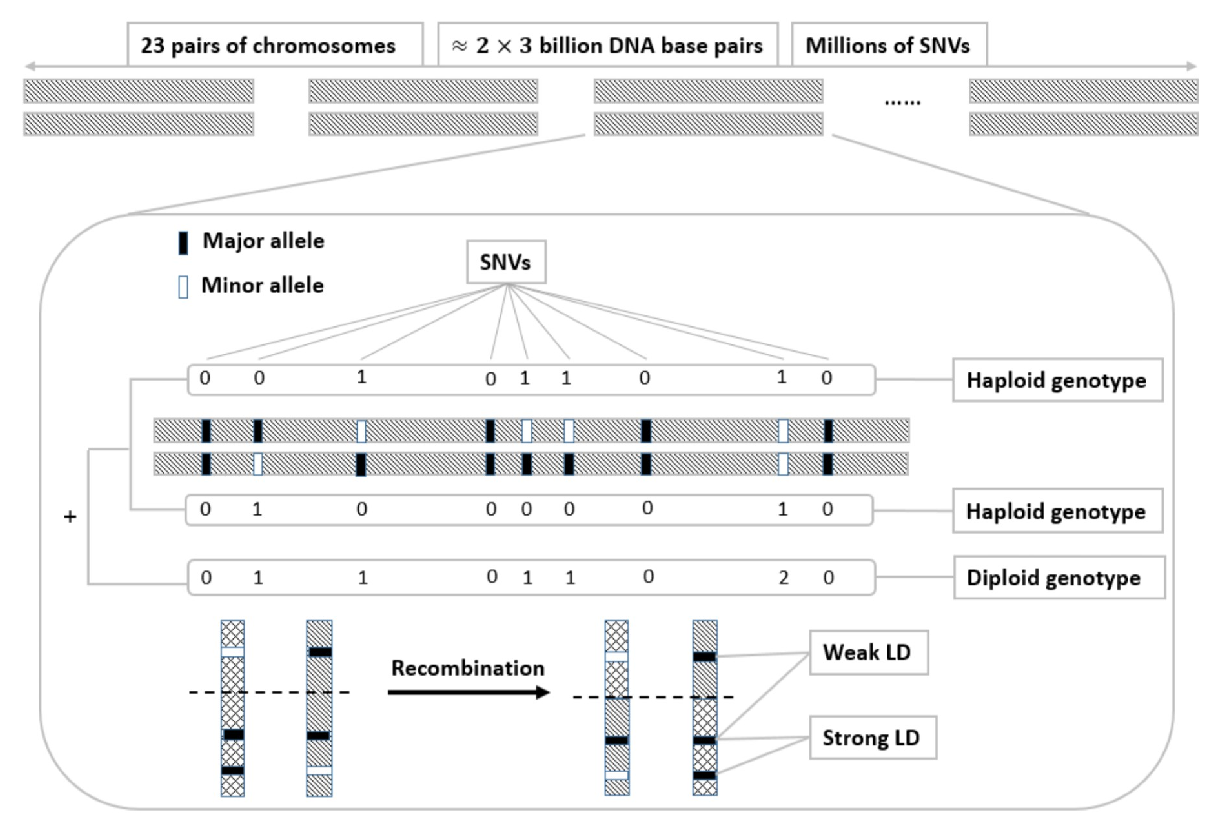
\includegraphics[width = 8.5cm]{./figures/Fig1-human-genomic-overview.eps}
	\caption{人类基因组概览\cite{samani2015quantifying}.
	}
	\label{fig:human-genomic-overview}
\end{figure}

为方便起见,让每个SNP的三个可能状态(分别为AA,Aa和aa)由0、1和2表示,具体取决于每个基因位点上次要等位基因的数量。

连锁不平衡(Linkage disequilibrium,LD)被定义为等位基因在两个或多个位点上的对应或非随机关联。这种关联是遗传机制的结果:如果有足够的进化时间,随机重组的出现将在所有位点产生等位基因的平衡分布。LD建模有几种方法。我们将重点介绍一种同时考虑参考基因型数据集和推荐率的混合方法。

在遗传过程中,重组是一个子过程,在这个过程中,一些DNA片段被分离并重新组合,形成新的等位基因组合。重组过程导致所有生物的遗传多样性。重组与LD是直观相关的。

\subsection{隐马尔科夫模型}

隐马尔可夫模型(HMM)\cite{rabiner1989tutorial,stamp2004revealing}是一种状态不可观测的统计马尔可夫模型,可以通过简单的动态贝叶斯网络表示。具体来说,在我们的讨论中采用了三个假设:(1)~$t$~时刻的状态是由某个状态为~$S_t$~ 隐藏的过程生成的;(2)该过程具有马尔可夫性;(3)隐藏的状态变量是离散的。
HMMs可用于表征诸如相似性、解码和学习等基本问题。 目前,HMMs在语音识别\cite{rabiner1989tutorial}、手写识别\cite{hu1996hmm}、基因预测\cite{durbin1998biological}等领域得到了广泛的应用。
本文考虑的问题在某种程度上类似于参数学习问题。由于在给定观测或发射序列的推理过程中,所有隐藏状态变量的后边缘都可以通过计算得到,因此我们考虑采用正向-反向算法。

\subsection{卷积神经网络}

卷积神经网络(Convolutional neural networks, CNNs)\cite{long2015fully,scutti2018what}最近已成为解决图像分类、分割和回归问题的一种流行方法。但是,尚未开发出回归CNN(RCNN)体系结构(其中最后一层是回归层的CNN)来预测基因型序列。与传统的分类分割问题不同,CNN的输出是离散值\cite{scutti2018what},而RCNN的输出是连续的。
在本工作中,我们设计了用于单倍型序列预测的RCNN架构,类似于缺失值预测的架构。首先,使用公共单倍型数据集来训练和测试我们的RCNN模型。建立模型后,通过将观察到的基因型逐步转化单倍型,进而推断隐藏的SNPs的基因型,将其应用于攻击个体的基因型序列。


\section{敌手模型和量化评估指标}\label{sec:adver}

\subsection{敌手模型}
\begin{figure}
	\centering
	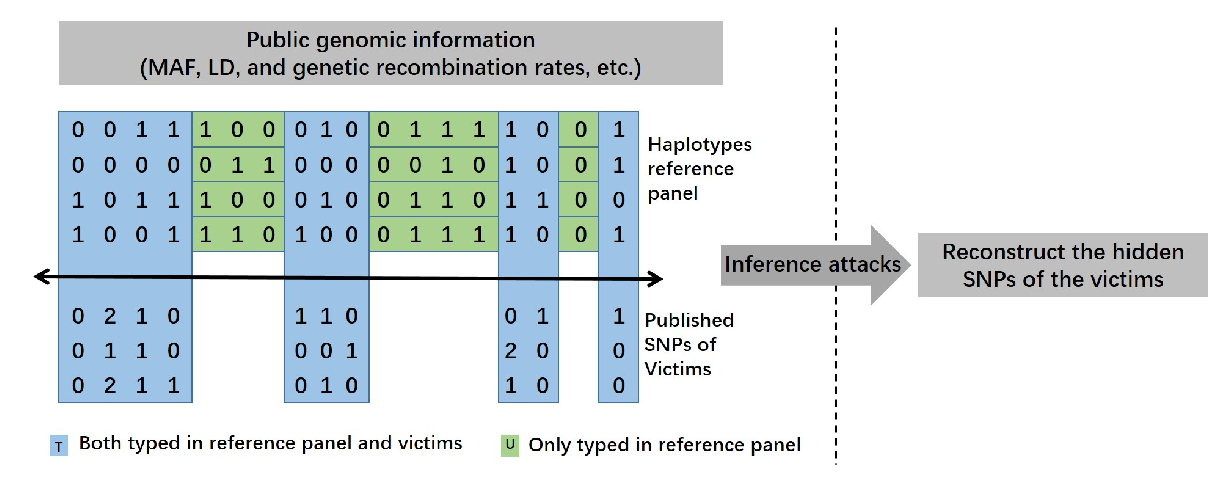
\includegraphics[width = 8.5cm]{./figures/Fig2-adversary-model.eps}
	\caption{敌手模型概览}
	\label{fig:adversary-model}
\end{figure}


本节提出的敌手模型考虑现实世界中涉及基因组数据共享的场景。在这种情况下,受害者捐赠他或她的SNP序列用于研究、医学测试或寻找亲属。由于隐私问题,受害者希望隐藏某些可能与遗传病或私人特征有关的敏感SNP。因此,受害人共享其原始SNP序列的变体~$\hat{X}=(\hat{x}_1,\hat{x}_2, ... , \hat{x}_n)$~, 其中~$\hat{x}_i =\{0,1,2\}$~,隐藏其中某些SNP。假设隐藏的SNP用$X_H$表示,可观察的SNP用~$X_O$~表示,发布的SNP用~$X=(x_1, x_2, ..., x_n)=X_H \cup X_O$~,其中~$x_i =\{-1,0,1,2\}$~,值~$x_i=-1$~表示$x_i\in X_H$是隐藏的SNP。假设可以观察受害者的已发布SNP~$X$~的敌手想要重构原始SNP序列~$\hat{X}$~。为此,敌手可以通过推理攻击侵入受害者的基因组隐私(例如获得其APOE基因状态\cite{nyholt_jim_2009}。要进行这样的推理攻击,敌手将收集一些公开可用的基因组信息\cite{IGSR_2019,IMPUTE2_Howie_2014},例如受害人所属人群的次要等位基因频率(MAF)、LD值、遗传重组率和单倍体基因型参考,如图~\ref{fig:adversary-model} 所示。

假设可访问的公共基因组信息用${INFOR}_{Pub}$表示,推断的SNP序列用$\bar{X}=(\bar{x}_1, \bar{x}_2,...,\bar{x}_n)$表示。基于基因型隐私的推理攻击推断的敌手模型$infer$可以形式化地表示为
\begin{align}\label{eq:adversary-model}
\bar{X} =& infer(X,{INFOR}_{Pub})  \nonumber \\
= & infer(X_H,H_O,{INFOR}_{Pub}).
\end{align}

更具体地说,推理攻击可以看作是给定已发布的SNP和公共基因组信息,计算每个隐藏SNP的条件边缘概率分布的过程,即
\begin{align}\label{eq:adversary-model-prob}
Prob(X=\{0,1,2\})=Prob(X|(X_O,{INFOR}_{Pub})).
\end{align}
对于每个隐藏SNP,其预测值是条件概率最高的那个值。
\subsection{量化评估指标}


为了量化敌手在基因组隐私推理方面的能力,需要使用Ayday等\cite{ayday2013personal}引入的\textit{基因组隐私度量}方法,从而评估对手通过推断攻击可以在多大程度上损害受害者的基因组隐私。就像Wagner
\cite{wagner2017evaluating}
所说的那样,有几种类型的基因组隐私度量适用于我们的探讨。在本文中,我们假设对手的目标是推断SNPs的值,我们只考虑个体实际拥有的SNPs。我们应用\textit{正规不正确性}(即敌手的不正确性),\textit{正规熵}(即敌手的不确定性)和\textit{正规互信息}(即受害者的隐私损失)来量化推理攻击模型的能力。

作为基因组隐私度量,\textit{正规不正确性}可以表示为
\begin{align}\label{eq:metric-correctness}
E=1- \frac{\sum_1^n \mid \bar{x}_j - \hat{x}_j \mid}  {\mid X_H \mid},
\end{align}

其中 $n$ 为属于受害者的SNP数量,$\bar{x}_j$ 为推断出的SNP在 $j$ 位点的基因型值,$\hat{x}_j$ 为SNP在 $j$ 位点的原始基因型值,$\mid X_H \mid$ 为属于受害者隐藏的SNP数量。

尽管不正确性是衡量隐私权的有力指标,但由于受害者SNP的原始值不可用,因此它并不适合许多场景。在这些情况下,我们需要其他指标。在本章中,我们采用\textit{正规熵}来表示敌手的不确定性,该度量可以根据所推导的SNPs的\textit{正规熵}来评估。特别地,
\begin{align}\label{eq:metric-entropy}
H = \frac{\sum_{j=1}^n \frac{H(X_j)}{log(3)}}{\mid X_H \mid},
\end{align}
其中$H(X_j)= -\sum_{\bar{x}_j=\in \{0,1,2\}}{p(\bar{x}_j)log(p(\bar{x}_j))}$ 为推断出的SNP在$j$位点的熵,$log(3)$为$j$位点SNP的最大熵,$\mid X_H \mid$ 为受害者的隐藏SNP数。

该度量标准根据敌手的能力而不是受害者的隐私损失来量化对手在其推理攻击中的置信度。为此,我们利用不确定性的递减来表示敌手在推理攻击前后对隐藏SNPs的不确定性的变化,互信息的概念 \cite{peng2016information}可以作为这种度量的基础。因此,我们使用正规互信息来量化敌手对受害者的平均隐私损失,即:
\begin{align}\label{eq:metric-mutual-information}
I = \frac{\sum_{j=1}^n \frac{H_{MAF}(X_j)}{log(3)}}{\mid X_H \mid}
- H,
\end{align}
其中$H_{MAF}(X_j) = -\sum_{x_j=\in \{0,1,2\}}{p_{MAF}(x_j)log(p_{MAF}(x_j))}$ 表示SNP在$j$位点的自然熵,$p_{MAF}(x_j)$为根据MAF数据集SNP发生的概率。公式Eq.~\ref{eq:metric-mutual-information} 中定义的度量表示推理攻击引起的熵变,从而可以度量推理攻击的能力,它还可以评估受害者在推理攻击时的基因组隐私损失。

\section{所提出的隐私分析方法}\label{sec:infer}

在这一节中,对于所使用的敌手模型,我们提出了两种推理攻击策略,一个是基于改进的HMM (iHMM)的隐私推理方法,另一个是基于RCNN模型的隐私推理方法。

\subsection{基于iHMM的隐私分析}

为了提高基因组隐私推断的性能,我们选择不像\cite{samani2015quantifying}中那样直接推断受害者的隐藏的SNP基因型,而是受IMPUTE2 \cite{howie2009flexible}基因型插补方法的启发,我们将攻击过程分为三个步骤:(1) 使用马尔可夫链蒙特卡罗抽样策略将观察到的受害者的SNPs分阶段转为单倍型;(2) 使用HMM模型分别推断每个受害者的隐藏单倍型对;(3)结合对每个受害者推断的单倍型对,形成推断的基因型序列。


在模型的详细构建中,我们将参照组和受害者的SNPs分为$T$(同时出现在参照组和受害者中的SNPs)和$U$(不出现在受害者中,但出现在参照组中的的SNPs)。我们假设有 $n$ 个受害者, $H_R^T$表示$T$中SNPs的参考单倍型集合,$H_V^T$ 表示受害者在$T$中观察到的SNPs的单倍型集合,$H_V^U$ 表示与$U$中SNPs相对应的受害者隐藏的单倍型集合,$H_V^T=\{H_{V,1}^T,H_{V,2}^T,..., H_{V,n}^T\}$ 表示$T$中与SNPs对应的受害者单倍型,其中$H_{V,i}^T$表示第$i$个受害者的单倍型对,$\rho$表示群组基因重组映射率。

更具体地说,基于iHMM的推理攻击可以分三个步骤进行,详细说明如下:
\begin{enumerate}
	\item[(1)] 敌手根据观察到的受害者的基因型,随机产生$H_V^T$ 的单倍型。然后,敌手通过多轮马尔可夫链蒙特卡罗迭代更新$H_V^T$ 中的单倍型。在每次迭代中,敌手通过从$P(H_{V,i}^T|G_{V,i}^T,H_{V,-i}^T,H_R^T,\rho)$ 中抽样来更新第$i$个受害者的阶段性单倍型对$H_{V,i}^T$ 。
	\item[(2)] 敌手通过基因重组模型利用HMM模型推断$H_V^U$中的单倍型。在每次迭代中,敌手根据条件分布$P(H_{V,i}^U|H_{V,i}^T, H_R^{T \cup U},\rho)$推断第$i$个受害者对应$U$中的SNPs的隐藏单倍型对$H_{V,i}^U$。 
	\item[(3)] 敌手把对每个受害者推断出来的单倍型对组合起来,得到受害者隐藏的SNPs的推断基因型。
\end{enumerate}

在步骤(1)中每次迭代的分阶段步骤中,抽样条件为$k$个最接近的单倍型,其结果由其到第$i$个受害者的汉明距离确定。利用基于重组过程的HMM模型计算条件分布,采用蒙特卡罗方法重构相空间。因为状态空间包含$H_R^T$中单倍型的所有状态和$H_{V,-i}^T$中当前猜测的单倍型,所以可以获得更多信息。

在步骤(2)中,HMM状态空间包含了所有参照单倍型$H_R^{T \cup U}$,此步骤类似于\cite{samani2015quantifying}中基于重组模型的过程,该模型受\cite{marchini2007new}的启发。然而,我们推断每个受害者的单倍型对,而不是直接推断基因型。

步骤(1)至(3)中描述的攻击策略与[\cite{samani2015quantifying}中描述的攻击策略不同,后者直接推断隐藏SNP的基因型值。在本文中,敌手结合了马尔可夫链蒙特卡洛抽样和HMM推理技术,改善了目标SNP序列的条件分布所获得的结果。

\subsection{基于RCNN的隐私分析}

基于RCNN的攻击也分为三个步骤,步骤(1)和(3)与基于iHMM的攻击是相同的,只有步骤(2)不同。同样地,敌手观察公开的基因组信息和受害者SNPs,将基因型分为单倍型,分别推断出隐藏的单倍型对,然后将推断出的单倍型对组合成基因型。在这里,我们将基于RCNN攻击的步骤(2)做说明如下。

我们构造RCNN的目标模型为
\begin{align}\label{eq:rcnn}
H_{V,i}^U  \leftarrow RCNN(H_{V,i}^T, H_R^{T \cup U}),
\end{align}
其中,给定一个参考单倍型集和一个基于观察到的SNPs的相位单倍型集,公式\ref{eq:rcnn}的目标是推断这些隐藏部分的值(即,0或1)。

由于受害者的公共参考单倍型和观察到的SNPs都属于同一群体(如CEU或CHS\cite{igsr2015which}),因此这些数据具有相同的特征,可以通过神经网络进行分析。

我们对参照数据$H_R^{T \cup U}$提出了一个RCNN模型,将这些数据分成两组:一组是训练集$H_{Rtrain}^{T \cup U}$,另一组是测试集$H_{Rtest}^{T \cup U}$。然后我们对最小值$min(\|H_{Rtest}^{ U} - \hat{H}_{Rtest}^{U}\|)$的目标选择最佳训练网络,其中$\hat{H}_{Rtest}^{U}$ 表示测试集的预测值。敌手可以使用这个优化的网络来推断受害者单倍型的隐藏值,具体过程如图\ref{fig:rcnn_infer} 所示。

\begin{figure}
	\centering
	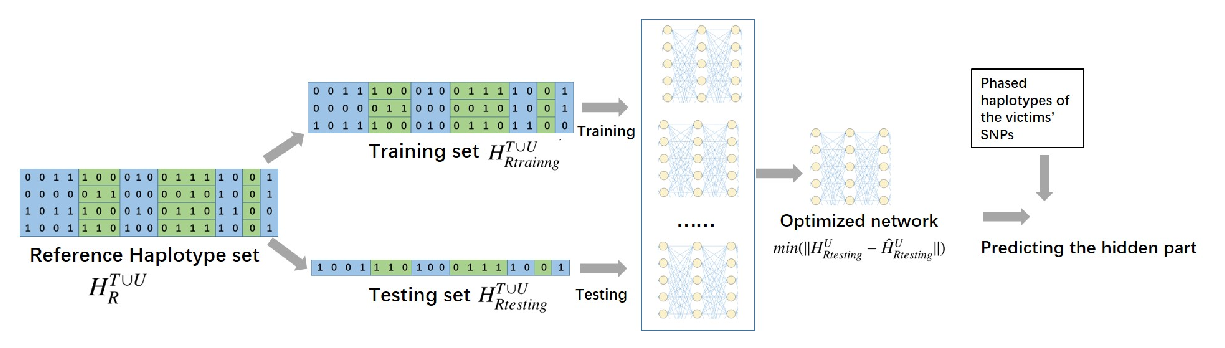
\includegraphics[width=14cm]{./figures/Fig3-RCNN-inference-attack.eps}\\
	\caption{基于RCNN的隐私分析模型}
	\label{fig:rcnn_infer}
\end{figure}


\begin{figure}
	\centering
	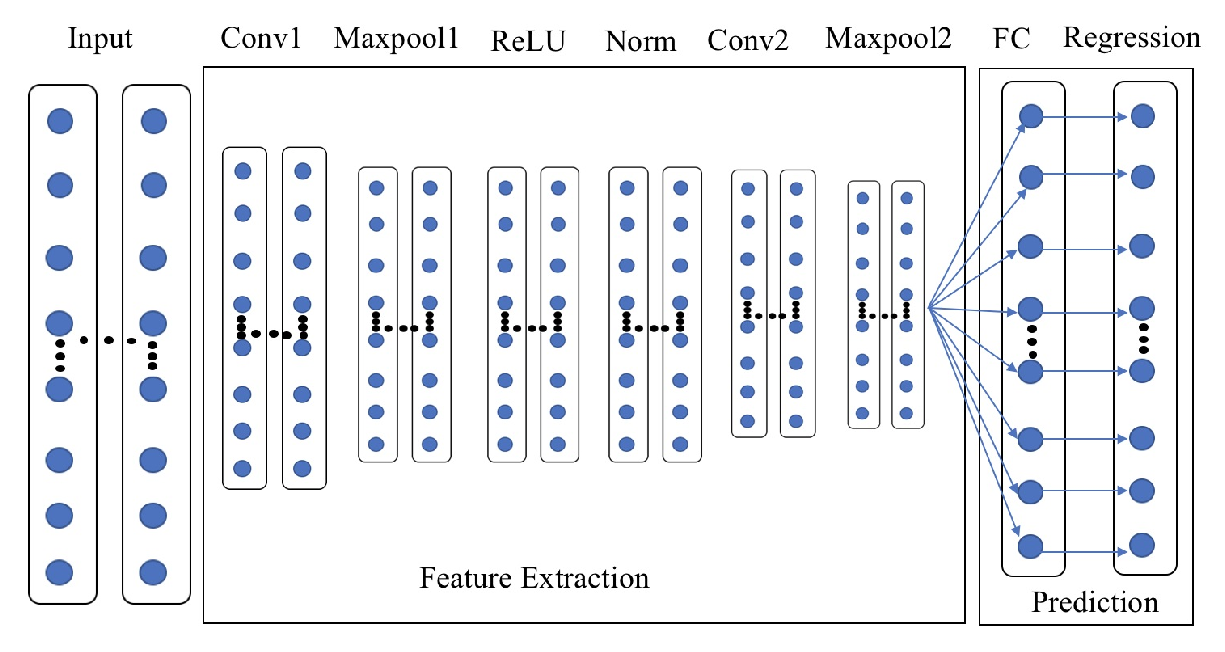
\includegraphics[width=8.5cm]{./figures/Fig4-RCNN-structure.eps}\\
	\caption{基于RCNN的基因隐私分析过程}
	\label{fig:RCNN}
\end{figure}
基于RCNN的基因隐私分析过程如图\ref{fig:RCNN}所示(其中,Conv为卷积层, NA为正规化层, FC为完全联通层),该过程包含8层网络,输入由观察到的SNPs的单倍型组成,最后一层回归层生成隐藏SNP序列的单倍体型值。最后一层是代表隐藏SNPs的单倍型的回归层。在训练阶段,RCNN能够提取基因型的影响因子,检验MES是否收敛。利用RCNN训练得到的分类器,可以对测试数据集中的隐藏SNP序列的单倍型值进行推测。
.) 

该网络可实现两项主要任务:特征提取和预测。该网络包括八层,两个卷积层(Conv1和Conv2)、两个最大池层(Maxpool1和Maxpool2)、一个整流线性单元层(ReLU)和一个归一化层(Norm),ReLU层减少了训练所需的时期数,但是因此其错误率比传统的双曲正切单位更高。规范层提高了通用性,降低了错误率。值得注意的是,ReLU层和Norm层并不会改变特征映射的大小。池化层汇总了相邻池化单元的输出。预测步骤完全由连接(FC)层和回归层执行。输入层由$8\times 1$个影响因子组成(1个月) ,Conv1和Conv2各自的过滤器大小($F$)为$1\times 1$ ,并且过滤器的数量($N$)为25,填充大小($P$)为0,Maxpool1和Maxpool2的步长($S$)为$2\times 2$。因此,在每个max池层之后,特征图的维数除以2。


为训练RCNN模型,我们最小化损失函数,使用均方误差(MSE)作为损失函数,其定义为
\begin{equation}
\text{Loss}=\frac{1}{N}\sum_{i=1}^{N}|d_{t}^{i}-d_{o}^{i}|^{2},
\end{equation}
其中$N$是数据集中的条目数,下标$i$表示数据集中的第$i$个条目。

\subsubsection{基于RCNN的单倍体型SNP值推测}
如图\ref{fig:RCNN},所示,一旦在Maxpool2层中提取了额外的特征,我们就可以将其连接到FC层,并将所有的特征压缩成一个维度。在训练过程中,如果在当前迭代次数未达到期望的MSE,则训练将继续进行,直到达到最大的迭代次数或所期望的MSE。如果达到最大迭代次数,则无论MSE值如何,训练过程都会停止。为了验证该方法的可行性和实用性,将测试数据集输入训练好的RCNN模型中,并利用该模型预测隐藏SNPs的单倍型,从而对总体性能进行评估


\section{实验及对比}\label{sec:resul}
在本节中,我们将根据各种指标评估我们提出的攻击方法的性能,并基于一组精心设计的实验的结果,将我们的结果与之前的工作进行比较。

\subsection{数据集}
在这些实验中,我们使用了来自HapMap项目\cite{thorisson2005international}第三阶段的数据集,该数据集在互联网上是公开的。在这个项目中,从世界各地11个不同的人群中收集匿名的基因组数据用于基因研究。在不失一般性的前提下,我们采用了2010年5月发布的北欧和西欧祖先(CEU)人群22号染色体的数据集。该数据集包含了个体的单倍型序列,并且还包括了这些群体的MAFs、成对LD值和重组率。我们将这些数据视为公共背景数据。此外,HapMap项目数据集中也包含165个个体的基因型序列。我们将使用这些数据作为选择的无关亲属的基因组数据。这个数据集也在文献\cite{samani2015quantifying}中使用过。
\subsection{结果}

在我们的实验中,我们随机隐藏受害者SNPs的不同百分比(从5\%到60\%),使用我们提出的攻击模型推断隐藏的SNPs,并根据第~\ref{sec:adver}节中所描述的三个指标量化基因组隐私结果。

首先,我们随机隐藏10\%的受害者的SNP,并使用不同的攻击模型评估敌手的推理能力。然后,我们进行20次实验,取每个指标对所有受害者的平均值。我们基于iHMM和RCNN模型评估攻击,敌手的不正确性、敌手的不确定性和受害者的隐私损失结果如表~\ref{tab:performance-10per}所示。在此表中,M1-LD,M2和RM分别表示文献 \cite{samani2015quantifying} 中基于一阶马尔可夫链(利用公开二元LD数据),二阶马尔可夫链和基因重组模型的推理攻击,而iHMM和 RCNN分别表示基于iHMM和RCNN模型的推理攻击。我们比较了错误率列中不同推理攻击的不正确性。我们的两种方法的结果都显示出总体上的不正确性明显降低,与RM方法相比,iHMM的性能更好,而RCNN的性能稍差。因为文献\cite{samani2015quantifying} 中的作者在他们的论文中没有考虑不确定性和隐私损失的度量,所以我们根据计算这两个度量的需要,改进他们的实验。所获得的结果表明,这两种度量方法同样适用于基因组隐私的测量。在表~\ref{tab:performance-10per}, 的正规熵列和正规隐私损失列中分别显示了不确定性和隐私损失方面的性能结果。结果表明,利用基于iHMM的推理攻击,敌手可以获得较低的不确定性,并获得更丰富的受害者隐私信息。

为了进一步支撑我们的比较结果,并与文献\cite{samani2015quantifying}中提出的实验保持一致,我们进行了另一个含有40\%隐藏SNPs的实验。性能结果如表~\ref{tab:performance-40per}所示,与表~\ref{tab:performance-10per}中的结果一致。

\begin{table}
	\caption{当10\%SNP序列被隐藏时,不同基因隐私分析攻击效果对比}
	\label{tab:performance-10per}
	\begin{tabular}{lccc}
		\hline
		& Error rate & Normalized entropy & Normalized privacy loss\\
		\hline
		M1-LD (Samani et al.) & 0.3356  & 0.4872 & 0.1864 \\
		M2 (Samani et al.)    & 0.2400  & 0.3419 & 0.3316\\
		RM (Samani et al.)    &  0.0578 & 0.069 & 0.6046 \\
		iHMM (Ours)          & 0.0085  &0.0295 & 0.6520 \\
		RCNN (Ours)          & 0.0753  &0.0973 & 0.5143\\
		\hline
	\end{tabular}
\end{table}


\begin{table}
	\caption{当40\%SNP序列被隐藏时,不同基因隐私分析攻击效果对比}
	\label{tab:performance-40per}
	\begin{tabular}{lccc}
		\hline
		& Error rate & Normalized entropy & Normalized privacy loss \\
		\hline
		M1-LD (Samani et al.) & 0.3623 & 0.4867 & 0.1873 \\
		M2 (Samani et al.)    & 0.2873 & 0.3489 & 0.3251 \\
		RM (Samani et al.)    & 0.0923 & 0.0902 & 0.5838 \\
		iHMM (Ours)          & 0.0136 & 0.0430 & 0.6342 \\
		RCNN (Ours)          & 0.1028 & 0.1345 & 0.5347\\
		\hline
	\end{tabular}
\end{table}

接下来,为了观察隐藏SNPs数量对不同推理攻击的影响,我们又进行了一组实验,实验中使用了不同比例(5\% - 60\%)的隐藏SNPs对LD、2阶马尔可夫链、重组模型、iHMM和RCNN攻击。敌手的不正确性、敌手的不确定性和敌手的基因组隐私损失结果分别如图~\ref{fig:error}、图~\ref{fig:uncertainty}和图~\ref{fig:privacyloss}所示

在图~\ref{fig:error}中,根据敌手的不正确性,我们展示了基于不同模型的推理攻击的结果。当受害者少量的SNPs被隐藏时,可以观察到这些攻击的推理能力会增加(即,受害者的SNPs暴露给敌手的越多,不正确性越低)。与之前的工作相比,我们提出的两种攻击模型在不正确性方面均显示出更好的推理能力。当隐藏更多SNPs(大于50\%)时,基于RCNN的攻击性能优于基于重组模型的攻击;当隐藏更少SNPs时(小于45\%)时,基于重组模型的攻击性能略差。

\begin{figure}
	\centering
	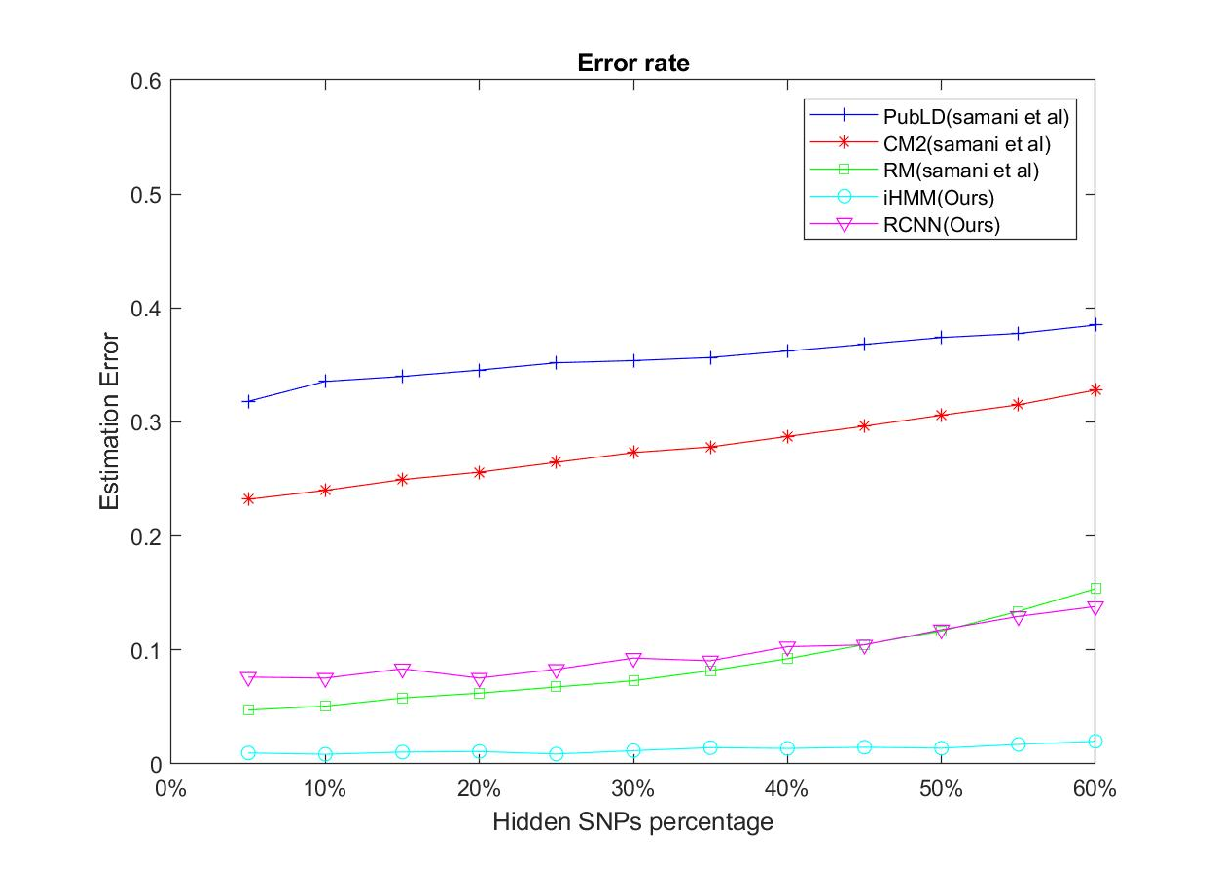
\includegraphics[width = 8.5cm]{./figures/Fig5-genomic-privacy-quantifying-incorrectness.eps}
	\caption{不同基因隐私分析模型的基因组隐私变化对比(攻击者错误率)}
	\label{fig:error}
\end{figure}

\begin{figure}
	\centering
	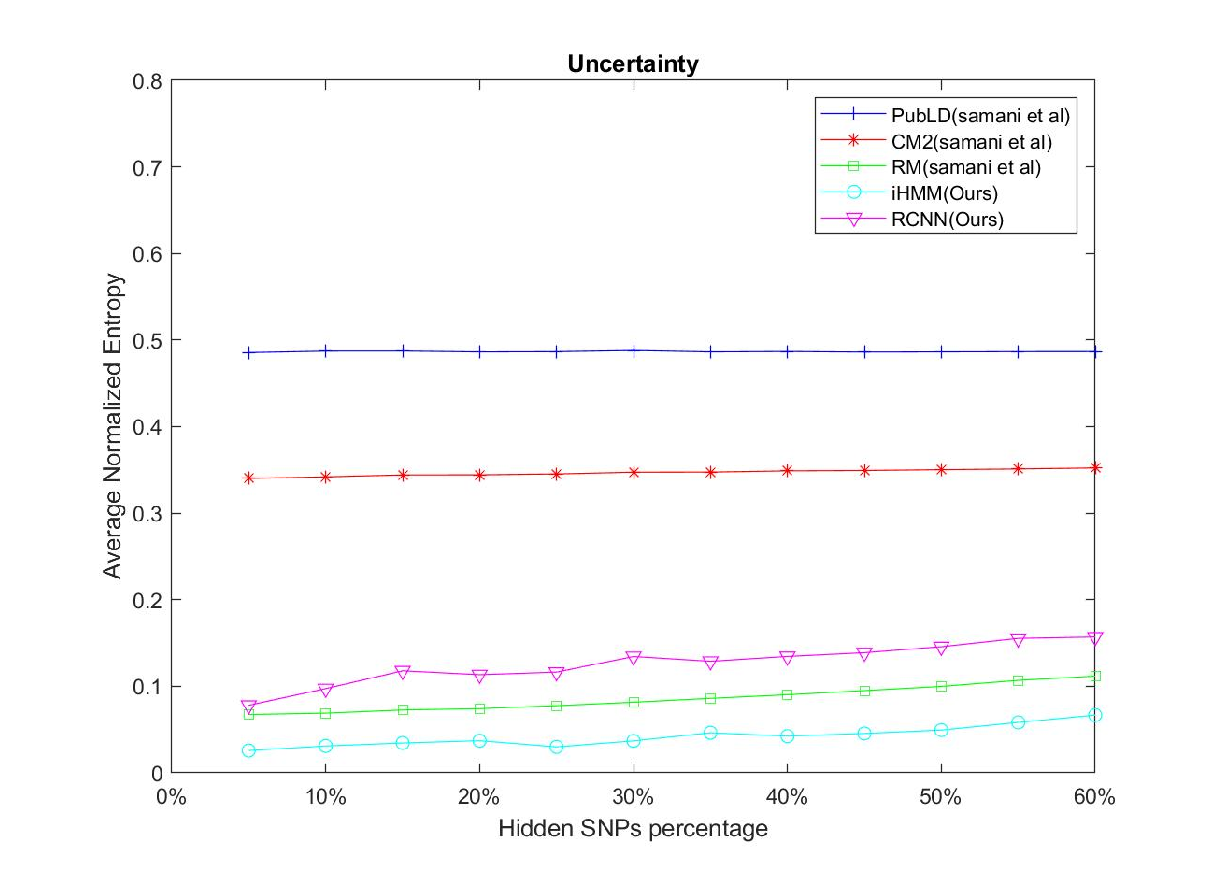
\includegraphics[width = 8.5cm]{./figures/Fig6-genomic-privacy-quantifying-uncertainty.eps}
	\caption{不同基因隐私分析模型的基因组隐私变化对比(攻击者不确定性)}
	\label{fig:uncertainty}
\end{figure}

在图~\ref{fig:uncertainty}中,我们根据敌手的不确定性显示了基于不同模型的推理攻击的结果。可以看出,当被敌手隐藏的SNPs越少时,这些攻击的推理能力越强(即,受害者的SNPs暴露给敌手的越多,不确定性越低),结果与图~\ref{fig:error}的结果一致。基于iHMM的攻击总是比其他攻击效果更好,而基于RCNN的攻击效果并非始终都是好的。

同样的,我们在图\ref{fig:privacyloss}中可以看到受害者隐私损失的结果。同样,当受害者隐藏的SNPS越少,这些攻击的推理能力就越强。(即受害者的SNPs暴露给敌手的越多,隐私损失越大)

\begin{figure}
	\centering
	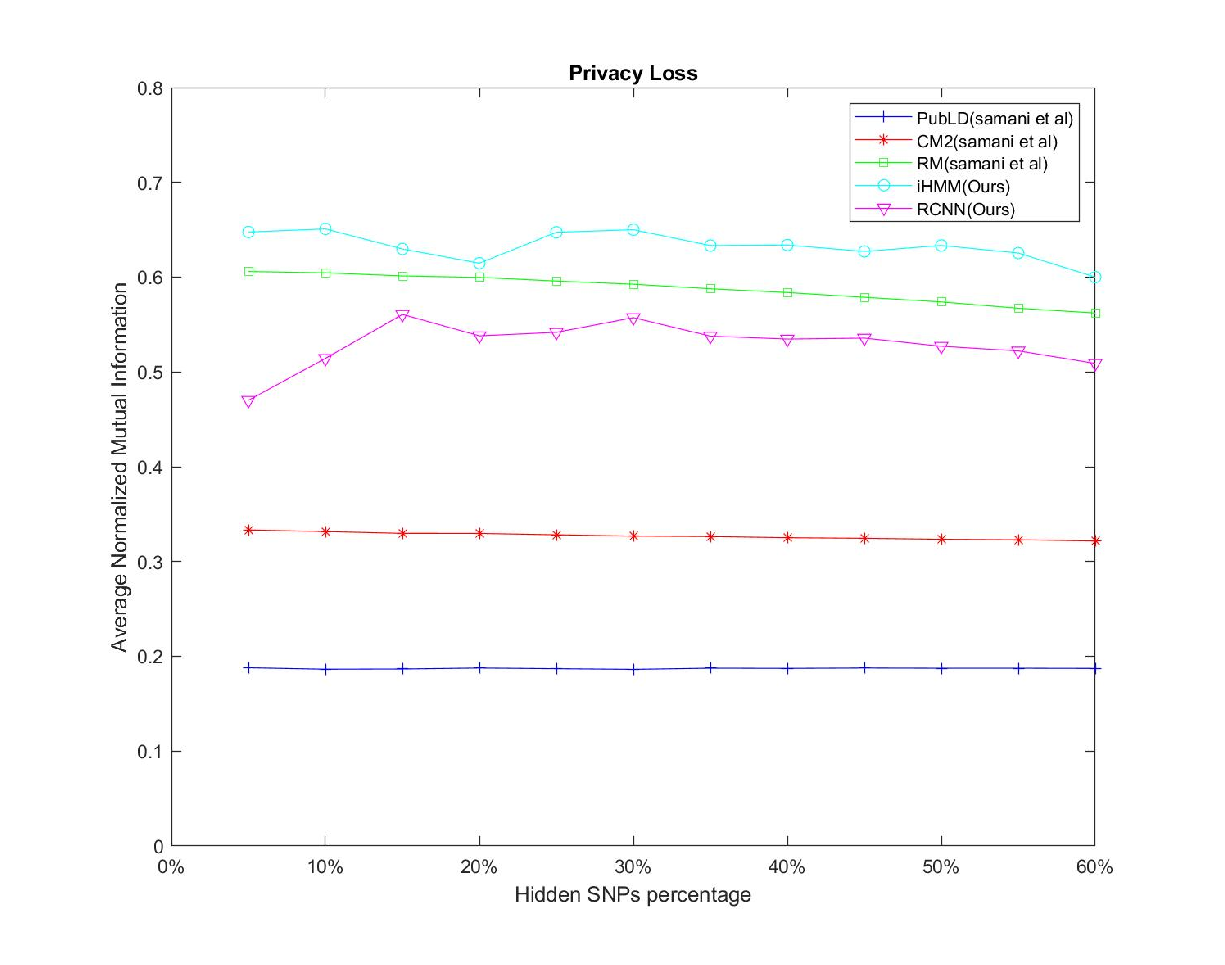
\includegraphics[width = 8.5cm]{./figures/Fig7-genomic-privacy-quantifying-privacyloss.eps}
	\caption{不同基因隐私分析模型的基因组隐私变化对比(受害人隐私损失角度)}
	\label{fig:privacyloss}
\end{figure}


\section{小结}\label{sec:concl}

在本章中,我们提出了几种攻击策略,通过改进的隐马尔可夫模型或回归卷积神经网络模型,在线结合公共基因组信息,从个体的部分SNP序列推断个体的基因型。研究表明,敌手能够准确、低不确定性和高隐私损失地推断出个体的私有隐藏SNP。实验表明,所提出的攻击扩展并显著改进了现有的工作。通过基于公开的基因组数据对个体基因组隐私进行量化,我们的工作可以帮助人们更好地理解当前基因组隐私面临的风险。
在未来,我们将进一步探索机器学习的潜力,将这种方法扩展到对亲属基因组隐私的攻击,并确定抵御基因组隐私攻击的合适方法。